%------------------------------------------------------------------------------------
%	PACKAGES AND OTHER DOCUMENT CONFIGURATIONS
%------------------------------------------------------------------------------------

\documentclass{article}

\usepackage{fancyhdr} % Required for custom headers
\usepackage{lastpage} % Required to determine the last page for the footer
\usepackage{extramarks} % Required for headers and footers
\usepackage[usenames,dvipsnames]{color} % Required for custom colors
\usepackage{graphicx} % Required to insert images
\usepackage{subcaption}
\usepackage{listings} % Required for insertion of code
\usepackage{courier} % Required for the courier font
% Optional Packages
\usepackage{amsmath}
\usepackage{amssymb}
\usepackage{float}
\usepackage{algorithm}
\usepackage[noend]{algpseudocode}


% Margins
\topmargin=-0.45in
\evensidemargin=0in
\oddsidemargin=0in
\textwidth=6.5in
\textheight=9.0in
\headsep=0.25in

\linespread{1.1} % Line spacing

% Set up the header and footer
\pagestyle{fancy}
\lhead{\hmwkAuthorName} % Top left header
\chead{\hmwkClass\ : \hmwkTitle} % Top center head
%\rhead{\firstxmark} % Top right header
\lfoot{\lastxmark} % Bottom left footer
\cfoot{} % Bottom center footer
\rfoot{Page\ \thepage\ of\ \protect\pageref{LastPage}} % Bottom right footer
\renewcommand\headrulewidth{0.4pt} % Size of the header rule
\renewcommand\footrulewidth{0.4pt} % Size of the footer rule

\setlength\parindent{0pt} % Removes all indentation from paragraphs


%------------------------------------------------------------------------------------
%	DOCUMENT STRUCTURE COMMANDS
%	Skip this unless you know what you're doing
%------------------------------------------------------------------------------------

% Header and footer for when a page split occurs within a problem environment
\newcommand{\enterProblemHeader}[1]{
	%\nobreak\extramarks{#1}{#1 continued on next page\ldots}\nobreak
	%\nobreak\extramarks{#1 (continued)}{#1 continued on next page\ldots}\nobreak
}

% Header and footer for when a page split occurs between problem environments
\newcommand{\exitProblemHeader}[1]{
	%\nobreak\extramarks{#1 (continued)}{#1 continued on next page\ldots}\nobreak
	%\nobreak\extramarks{#1}{}\nobreak
}

\setcounter{secnumdepth}{0} % Removes default section numbers
\newcounter{homeworkProblemCounter} % Creates a counter to keep track of the number of problems
\setcounter{homeworkProblemCounter}{0}

\newcommand{\homeworkProblemName}{}
\newenvironment{homeworkProblem}[1][Problem \arabic{homeworkProblemCounter}]{ % Makes a new environment called homeworkProblem which takes 1 argument (custom name) but the default is "Problem #"
	\stepcounter{homeworkProblemCounter} % Increase counter for number of problems
	\renewcommand{\homeworkProblemName}{#1} % Assign \homeworkProblemName the name of the problem
	\section{\homeworkProblemName} % Make a section in the document with the custom problem count
	\enterProblemHeader{\homeworkProblemName} % Header and footer within the environment
}{
	\exitProblemHeader{\homeworkProblemName} % Header and footer after the environment
}

\newcommand{\problemAnswer}[1]{ % Defines the problem answer command with the content as the only argument
	\noindent\framebox[\columnwidth][c]{\begin{minipage}{0.98\columnwidth}#1\end{minipage}} % Makes the box around the problem answer and puts the content inside
}

\newcommand{\homeworkSectionName}{}
\newenvironment{homeworkSection}[1]{ % New environment for sections within homework problems, takes 1 argument - the name of the section
	\renewcommand{\homeworkSectionName}{#1} % Assign \homeworkSectionName to the name of the section from the environment argument
	\subsection{\homeworkSectionName} % Make a subsection with the custom name of the subsection
	\enterProblemHeader{\homeworkProblemName\ [\homeworkSectionName]} % Header and footer within the environment
}{
	\enterProblemHeader{\homeworkProblemName} % Header and footer after the environment
}


%=================================================================

%------------------------------------------------------------------------------------
%	NAME AND CLASS SECTION
%------------------------------------------------------------------------------------

\newcommand{\hmwkTitle}{Assignment\ \#3} % Assignment title
\newcommand{\hmwkClass}{CSC321} % Course/class
\newcommand{\hmwkAuthorName}{Xiangyu Kong} % Your name
\newcommand{\hmwkUTorId}{kongxi16} % UTorID

%------------------------------------------------------------------------------------
%	TITLE PAGE
%------------------------------------------------------------------------------------

\title{
	\vspace{2in}
	\textmd{\textbf{\hmwkClass:\ \hmwkTitle}}\\
	%	\normalsize\vspace{0.1in}\small{Due\ on\ \hmwkDueDate}\\
	\vspace{0.1in}
	\vspace{3in}
}

\author{\textbf{\hmwkAuthorName} \\ \textbf{\hmwkUTorId}}

% Insert date here if you want it to appear below your name
\date{\today} 

%------------------------------------------------------------------------------------

\begin{document}
	
	\maketitle
	\clearpage
	
	%---------------------------------------------------------------------------------
	%	PROBLEM 1
	%---------------------------------------------------------------------------------
	\begin{homeworkProblem}
		%		\noindent \textit{Question}
		\begin{enumerate}
			\item 
			The model will not perform well on long sequences. This is because after the encoder compresses the long sequence of inputs into the fixed length vector $h_v$, $h_v$ will have to convey much more information. This makes the vector harder to interpret for the decoder layer, and the decoder will less likely give a correct result.
			
			\item 
			The added words are `team', `problematic', `ink', `obviously', `shy', `philosophical', and `supercalifragilisticexpialidocious'
			
			The predicted results are shown in below.
			
			As we can see, for shorter words like team and ink, the translator does a good job. However, for longer words like `problematic', `philosophical' and `supercalifragilisticexpialidocious', the translator does a very poor job.
			
			\begin{lstlisting}[caption = Translated Results]
	team --> eamtay
	problematic --> opserarcepray
	ink --> inkway
	obviously --> odloy-eylway
	shy --> ytsay
	philosophical --> isorecarcalclay
	supercalifragilisticexpialidocious --> afessfsesesssipicici
			\end{lstlisting}
		\end{enumerate}
		
	\end{homeworkProblem}
	\clearpage
	
	%---------------------------------------------------------------------------------
	
	
	%---------------------------------------------------------------------------------
	%	PROBLEM 2
	%---------------------------------------------------------------------------------
	\begin{homeworkProblem}
		
		\begin{enumerate}
			\item 
			The problem with teacher forcing is that during training, the decoder are given in ground truth token as input to next time unit. However, when training, the decoder has to predict the next letter given the previous prediction. If the previous prediction is incorrect, then the error will be enlarged through time because every time step, the decoder is predicting based on a false previous input.
			
			\item 
			A solution would be to generate a token that contains necessary and important information for predicting the next result to use as the next time step's input instead of simply using the previous result.
		\end{enumerate}
		
		
	\end{homeworkProblem}
	\clearpage
	
	%---------------------------------------------------------------------------------
	
	
	%---------------------------------------------------------------------------------
	%	PROBLEM 3
	%---------------------------------------------------------------------------------
	\begin{homeworkProblem}
		%		\noindent \textit{Question}
		See model.py for implementation
		
	\end{homeworkProblem}
	
	
	%---------------------------------------------------------------------------------
	
	
	%---------------------------------------------------------------------------------
	%	PROBLEM 4
	%---------------------------------------------------------------------------------
	\begin{homeworkProblem}
		%		\noindent \textit{Question}
		See model.py for implementation
		
	\end{homeworkProblem}
	\clearpage
	
	%---------------------------------------------------------------------------------
	
	
	%---------------------------------------------------------------------------------
	%	PROBLEM 5
	%---------------------------------------------------------------------------------
	\begin{homeworkProblem}
		%		\noindent \textit{Question}
		The words and their translations are given in the listing below. As we can see, simple short words are more likely to produce correct translations. For example, ``cake", ``labour", ``drink" and ``phone" all have the right translations and the visualizations are given in Fig\ref{fig:5.1}. In the visualizations, we see that the network goes linearly through the letters after the first consonant (block). This shows that the network can correctly capture these simple structures of the word.
		
		However, the network starts to make mistakes when it gets unusual and long words. For example, ``p-value", ``well-done", ``anthropocene", etc are translated incorrectly. The visualizations are given in Fig\ref{fig:5.2}. We can see that for ``p-value", the network understands that ``p" should be placed at the back but it does not know what to do with the dash ``-". For ``anthropocene", the network successfully understands that no letter needs to be placed at the back but gets lost after the second ``a". This is because the network was not trained enough with these specific structures and thus does not know how to translate them.
		
		\begin{lstlisting}[caption = words and predictions]
	roomba --> ooodrray
	cake --> akecay
	labour --> abourlay
	drink --> inkdray
	phone --> onephay
	bouquet --> ouquerbay
	anthropocene --> anthanthayentay
	p-value --> -ueyeydray
	well-done --> elay-onelyyday
	thimolystically --> ipthallystitesthay
	supercalifragilisticexpialidocious --> upercacalicalicaalic
		\end{lstlisting}
		
		\begin{figure*}[!ht]
			\begin{subfigure}{.5\textwidth}
				\centering
				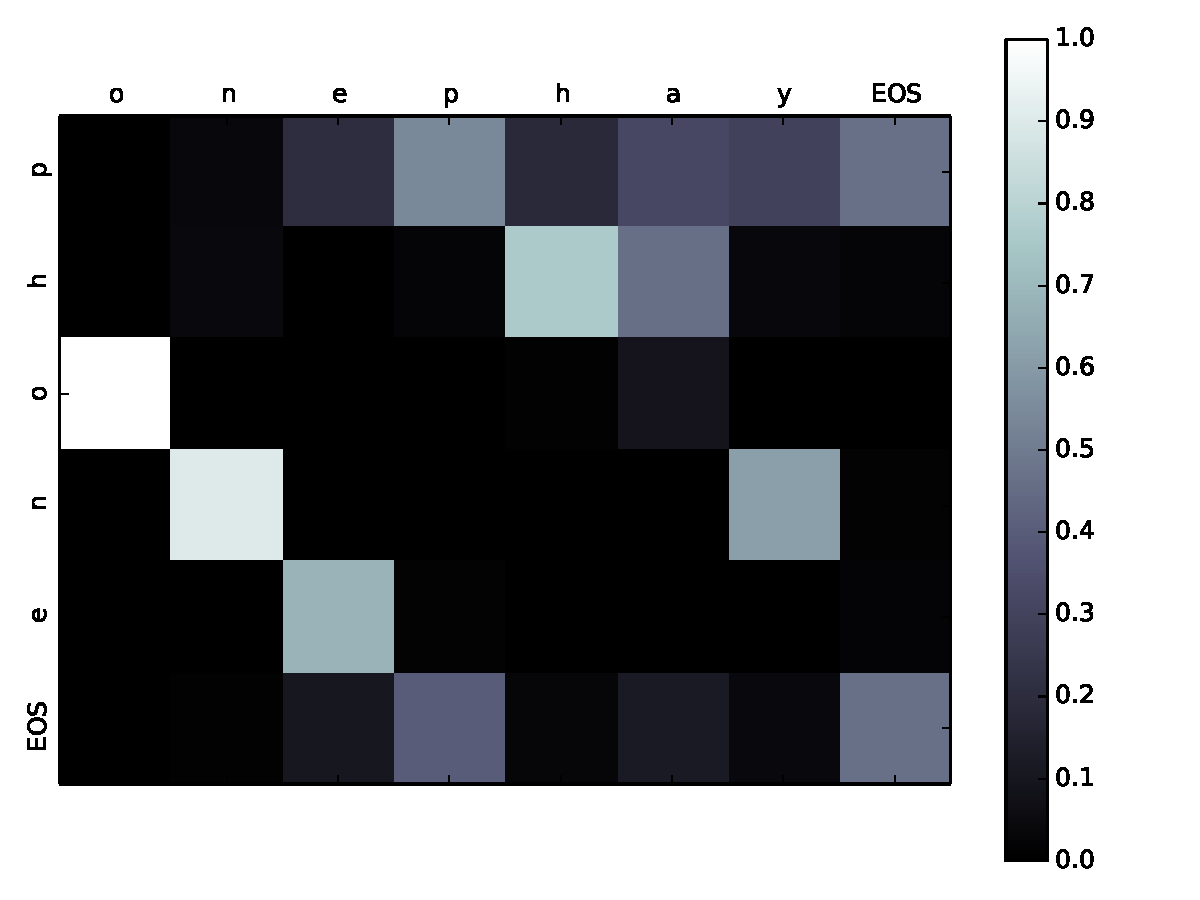
\includegraphics[width=.8\linewidth]{images/5/phone.pdf}
				\caption{phone}
				\label{fig:5.11}
			\end{subfigure}
			\begin{subfigure}{.5\textwidth}
				\centering
				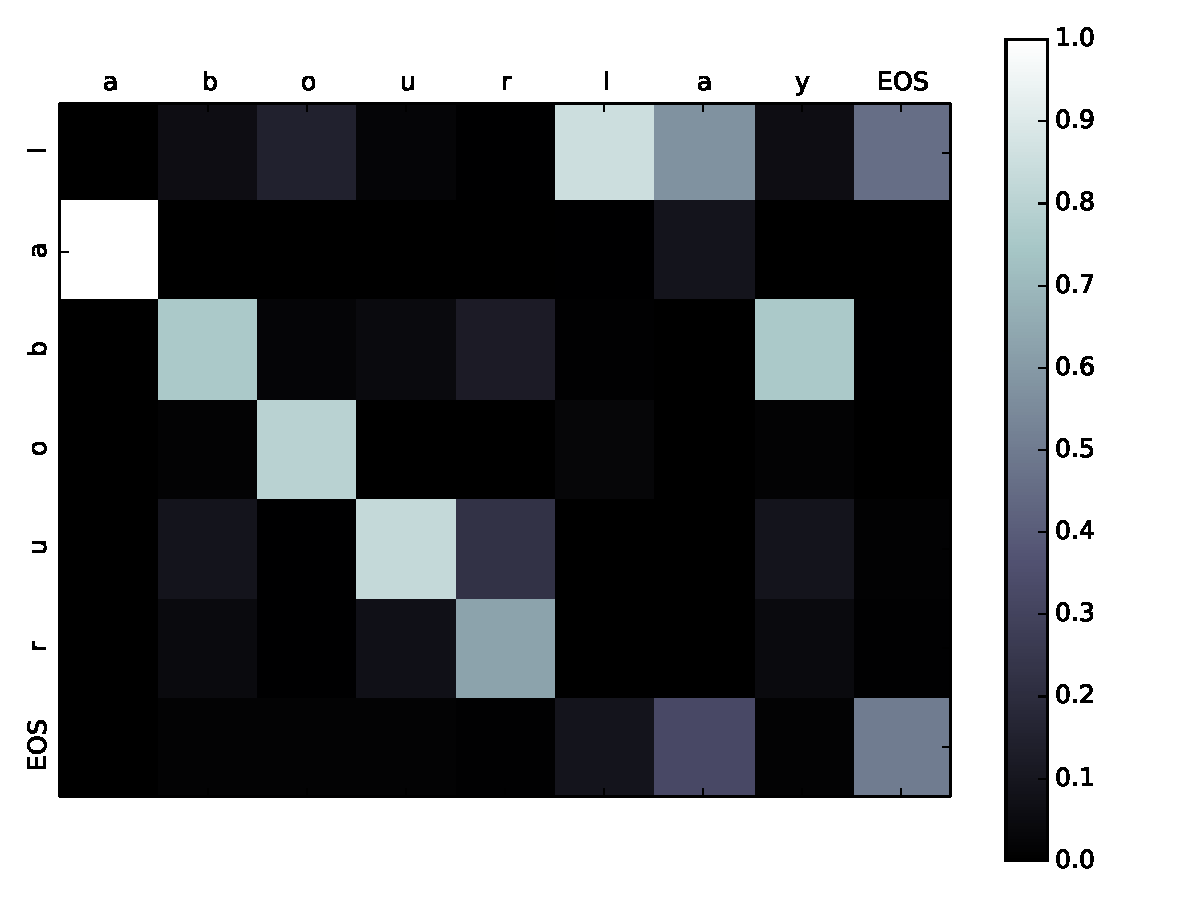
\includegraphics[width=.8\linewidth]{images/5/labour.pdf}
				\caption{labour}
				\label{fig:5.12}
			\end{subfigure}
			\caption{Correct Visualizations}
			\label{fig:5.1}
		\end{figure*}
	
		\begin{figure*}[!ht]
			\begin{subfigure}{.5\textwidth}
				\centering
				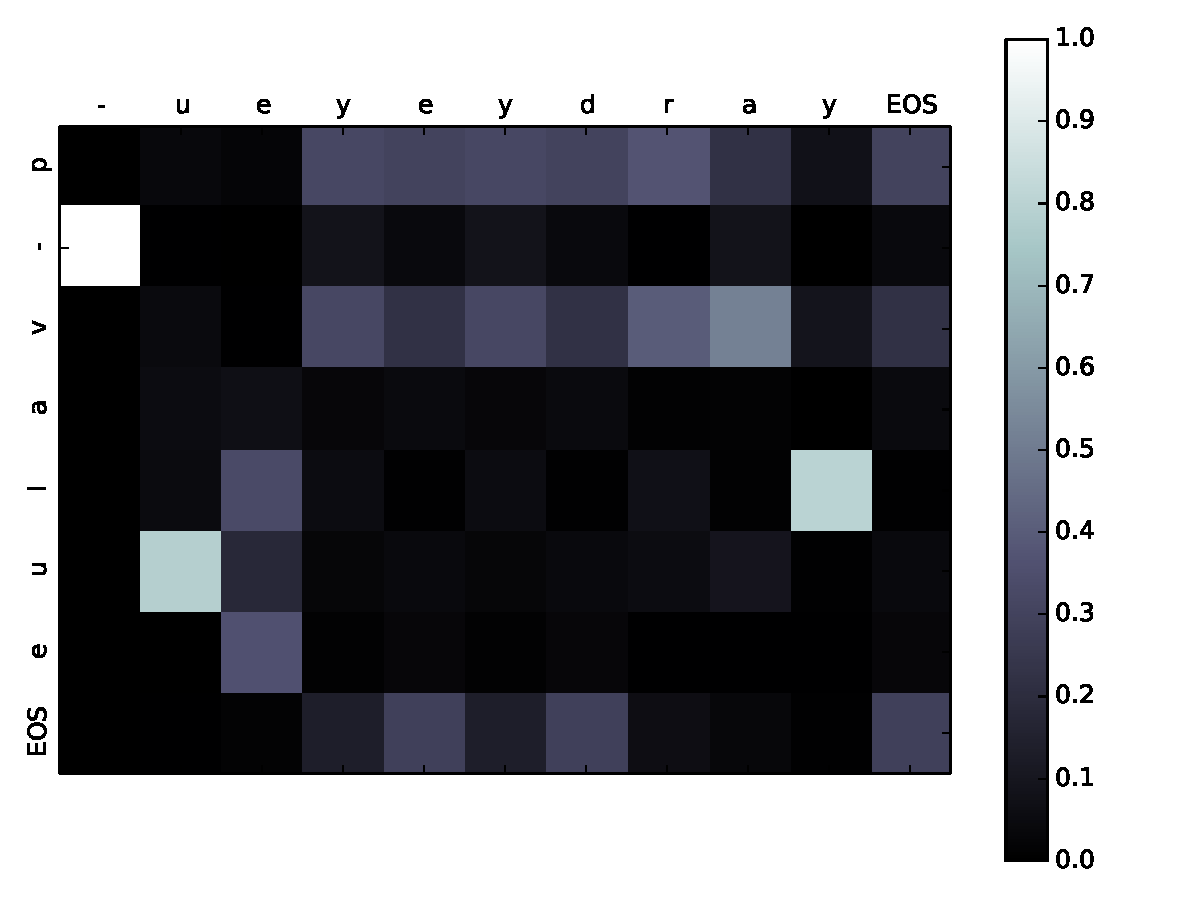
\includegraphics[width=.8\linewidth]{images/5/p-value.pdf}
				\caption{p-value}
				\label{fig:5.21}
			\end{subfigure}
			\begin{subfigure}{.5\textwidth}
				\centering
				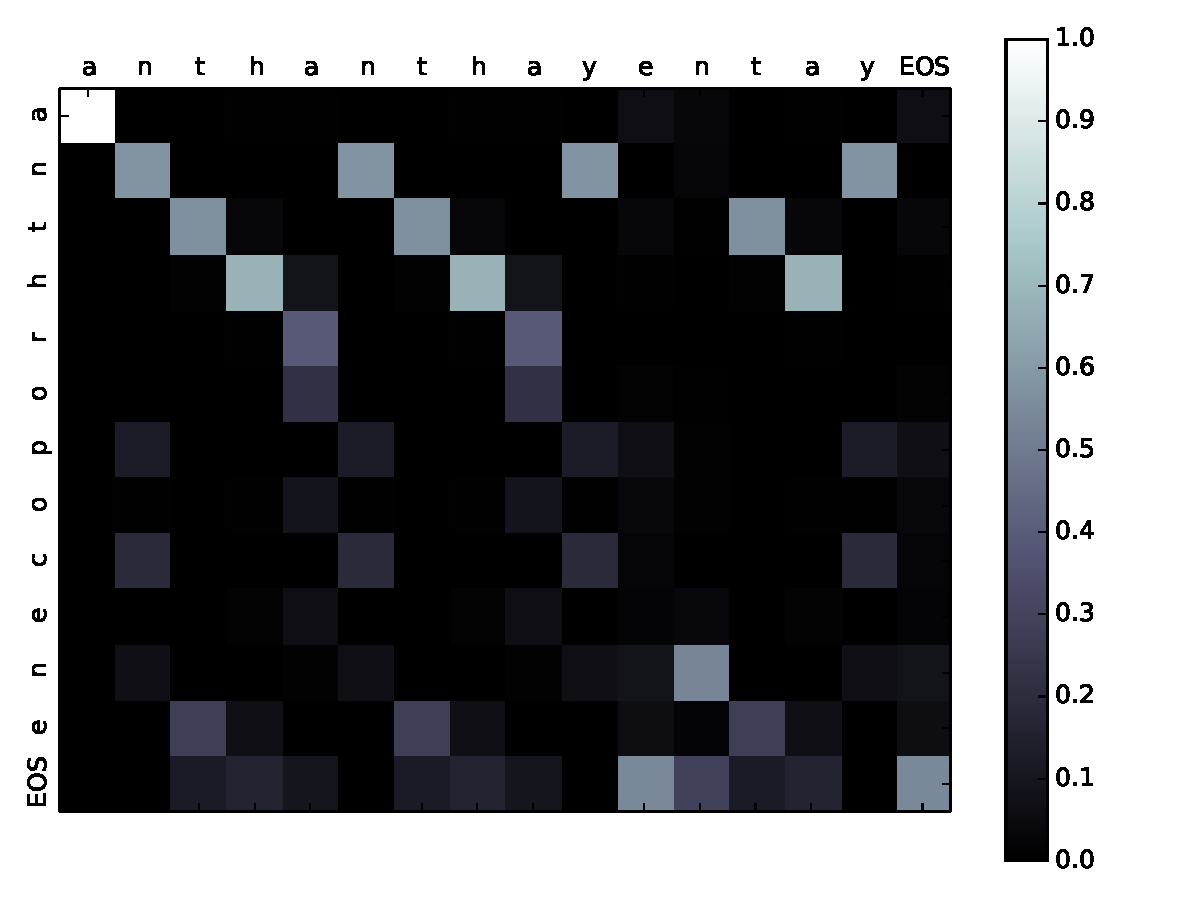
\includegraphics[width=.8\linewidth]{images/5/anthropocene.pdf}
				\caption{anthropocene}
				\label{fig:5.22}
			\end{subfigure}
			\caption{Incorrect Visualizations}
			\label{fig:5.2}
		\end{figure*}
		
	\end{homeworkProblem}
	\clearpage
	
	%---------------------------------------------------------------------------------
	
\end{document}